\documentclass{standalone}
\usepackage{tikz}
\usepackage{pgf}
\usepackage{amsmath}
\usetikzlibrary{decorations.pathreplacing}
\usetikzlibrary{calc}
\usetikzlibrary{angles,quotes}
\begin{document}
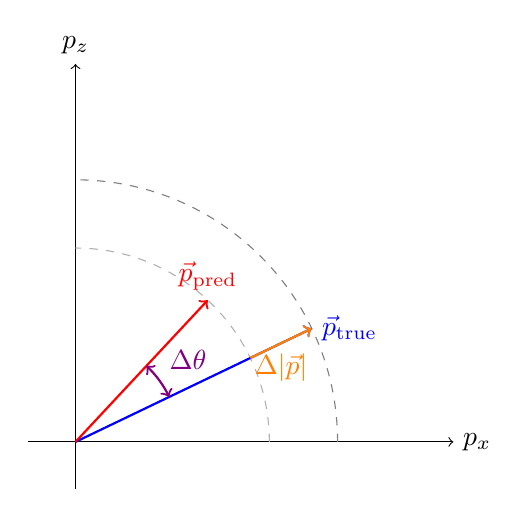
\begin{tikzpicture}[scale=1.2]

    % Axes
    \draw[->] (-0.5,0) -- (4,0) node[right] {$p_x$};
    \draw[->] (0,-0.5) -- (0,4) node[above] {$p_z$};

    \coordinate (origin) at (0,0);
    \coordinate (true) at (2.5,1.2);
    \coordinate (pred) at (1.4,1.5);

    % Magnitudes
    % |true| = sqrt(2.5^2 + 1.2^2) = sqrt(6.25+1.44) = sqrt(7.69) ~ 2.774
    % |pred| = sqrt(1.4^2 + 1.5^2) = sqrt(1.96+2.25) = sqrt(4.21) ~ 2.052
    % Unit vector of true direction: (2.5/2.774, 1.2/2.774) ~ (0.9013, 0.4327)
    % Pred magnitude endpoint along true direction: 2.052 * (0.9013, 0.4327) ~ (1.850, 0.888)

    % Dashed circle arc showing true magnitude
    \draw[dashed, gray] (2.774,0) arc[start angle=0, end angle=90, radius=2.774];

    % Dashed circle arc showing pred magnitude
    \draw[dashed, gray!60] (2.052,0) arc[start angle=0, end angle=90, radius=2.052];

    % True vector
    \draw[thick,blue,->] (origin) -- (true) node[right] {$\vec{p}_{\text{true}}$};
    % Predicted vector
    \draw[thick,red,->] (origin) -- (pred) node[above] {$\vec{p}_{\text{pred}}$};

    % Point on true direction at pred magnitude, to show magnitude difference
    \coordinate (predOnTrue) at (1.850, 0.888);

    % Magnitude difference: brace along the true direction
    \draw[thick, orange, ->] (predOnTrue) -- (true)
        node[midway, below, orange] {$\Delta |\vec{p}|$};

    % Angle arc between true and pred

    % Angle difference arc between the two vectors
    % true angle ~ 25.6 deg, pred angle ~ 47.0 deg
    \draw[thick, violet, <->]
        (1.1*0.9013, 1.1*0.4327) arc[start angle=25.6, end angle=47.0, radius=1.1]
        node[midway, above right] {$\Delta\theta$};

\end{tikzpicture}
\end{document}